\section{Introduction}\label{sec:intro}

\subsection{Biological question of interest}\label{subsec:biol}

\subsubsection{Background}
%	\textbf{What is gene expression}\\

Gene is a piece of DNA that encodes a functional RNA or protein product, and is the basic physical
and functional unit of heredity. The process by which genes are used to synthesize functional gene
products is called \textit{gene expression}.  A gene is considered to be expressed in a cell or
group of cells when a gene product is detected.
These products can be transcribed messenger RNA (mRNA) and proteins for protein coding genes, or
functional RNA species such as transfer RNA (tRNA) or small nuclear RNA (snRNA) for non-protein
coding genes.
Since the information encoded in a gene is first transcribed into RNA molecules, which is then used
to make functional gene products, the RNAs transcribed
in a certain condition reflects the current state of the cell.

% In molecular biology, the central dogma has been described as ``DNA makes RNA and RNA makes
%protein" \citep{leavitt2004deciphering}. 


% In RNA-Seq experiment, the expression
%level of a gene is reflected by the relative abundance of the corresponding transcriptome, which is
%in turn measured by the number of fragments  mapped to the reference genome. 




\textbf{Why do people do expression analysis?}\\
In a typical gene expression experiment, researchers are usually interested in comparing expression
levels of one or more genes from different sources. Factors for comparison can be
\textit{before vs
	after} effect in a drug treatment, \textit{tumor vs normal} tissues in clinical study, or
\textit{wild type vs mutant} strains in plant research. Another important factor is time-course,
where cells/tissues at different stages are sampled with the purpose of discovering temporal pattern
of gene expression. There are many other types of experiment, each with specific factors of interest
to be studied.


\textbf{What tools do people use to measure gene expression?}\\
The  expression levels of a gene can be measured using techniques such as
complementary DNA (cDNA) libraries, microarray analysis, RNA fingerprinting by arbitrary primed PCR
(RAP-PCR), expressed sequence tag (EST) sequencing, serial analysis of gene expression (SAGE), and
RNA sequencing (RNA-Seq) (see \cite{casassola2013gene} for a review).
% imaging, amplification, probe hybridization or sequencing-based detection methods .
RNA-Seq, also known as \textit{whole transcriptome shotgun sequencing}
\citep{morin2008profiling}, is a next-generation sequencing (NGS) technology used to uncover the
presence and quality of RNA in a biological sample.  It is rapidly becoming technology of choice
for transcriptome profiling over the past few years. 
The standard procedure of an RNA-Seq experiment runs as follows 
\citep{finotello2015measuring}: first, the RNAs in the biological sample are fragmented and
reverse-transcribed into cDNAs; second, the cDNA fragments are amplified and sequenced in a
high-throughput sequencing platform (e.g., Illumine 3000, \url{http://www. illumina.com}) to
generate (up to) hundreds of millions of reads; third, those reads are mapped to a reference
genome
or a reference transcriptome.
It is the number of reads aligned to each gene (referred to as ``read count") on the reference
genome/transcriptome that quantifies the genes' expression levels.  


\textbf{pros and cons about RNA-Seq}\\
RNA-Seq technology offers several key advantages over other methods \citep{wang2009rna}, the most
important of which are that it does not require prior knowledge of an organism for detecting
transcripts,  and that it is sensitive to genes expressed at either low or higher levels and thus
provides higher dynamic range. The sequencing of RNA allows researchers to study the entire
transcriptome of a species using only small amount of RNA. It has been demonstrated that a
coordinated effort between RNA-Seq and real time PCR (RT-PCR) is one of the most effective ways to
identify new exons \citep{howald2012combining}. However, one major challenge of this technique is
data processing: RNA-Seq experiment produces a huge amount of reads (up to hundreds of
millions per sample) and obtaining the expression profiles requires fast read mapping tools as well
as a lot of computing resource
\citep{langmead2009ultrafast,li2010fast}.



\textbf{A workflow of pre-processing RNA-Seq data}\\
Preprocessing RNA-Seq data consists of two main steps: 1) mapping reads to the reference
genome/transcriptome, and 2) summarizing read counts at given genomic feature (e.g., exon, gene or
transcript) level. Read mapping is the first computational, and usually, the most time-consuming
step in RNA-Seq data analysis. Currently, there are many alignment tools available, for example,
Bowtie \citep{langmead2012fast,langmead2009ultrafast}, BWA \citep{li2013aligning,li2009fast},
Subread \citep{shi2013subread} and STAR \citep{dobin2013star}. In all situations, an index of either
the reference genome/transcriptome or the reads are built at the beginning using hash tables or Burrows-Wheeler
transform (BWT) \citep{burrows1994block}. The index allows fast retrieval of the set of positions in
the reference sequence where the reads are more likely to align. Once those positions are decided,
alignment is performed in the candidate regions. The precision and speed of the alignment is mainly
determined by the algorithm used in the alignment tool (see \citep{hatem2013benchmarking} or
\cite{li2010survey} for a review). After the reads have been aligned, the numbers of reads mapped to
each unit of a specified genomic feature are counted, giving the estimate of the corresponding
expression profiles. This can be done using HTSeq \cite{anders2010htseq} or featureCounts
\citep{liao2013featurecounts}, among other options. Finally, a read count matrix is
obtained with each row representing a genomic feature unit and each column corresponding to a biological
sample. 

In this research work, we assemble an in-house pipeline to process RNA-Seq data sets based on the R \citep{Rpackage}
platform.
This pipeline, modified from a standard procedure given by \citet{anders2013count},   is designed to work
for sequencing data available at the \textit{National Center for Biotechnology Information} (NCBI,
\url{http://www.ncbi.nlm.nih.gov/}). It uses SRA (Sequence Read Archive) Toolkit
\citep{leinonen2010sequence} to convert SRA files to FASTQ files, \verb|Subread| aligner
\citep{liao2013subread} to map reads to the reference genome, and then \verb|featureCounts| \citep{liao2013featurecounts} to summarize
counts (see Figure \ref{fig:flowchart} for the work flow). We will use it to process multiple
RNA-Seq data sets in Chapter \ref{chap1}.
\begin{figure}[!ht]
	\centering
	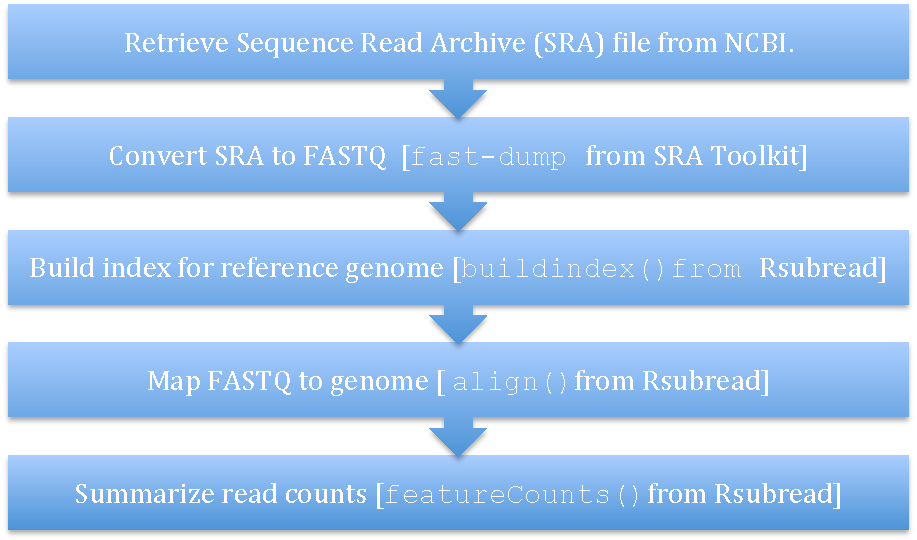
\includegraphics[width=0.7\linewidth]{Figures/flowchart.pdf}
	\caption{Work flow of data preprocessing: from raw reads sequencing data to read counts. Raw data
		in this workflow are retrieved from the NCBI. Data processing is based on two softwares SRA
		Toolkit
		\citep{leinonen2010sequence} 
		and Rsubread aligner \citep{liao2013subread}).}
	\label{fig:flowchart}
\end{figure}	



\subsubsection{Statistical issues}
The statistical analysis beginning from the read count matrix consists of three major parts: 1)
normalization---adjusting for sources of bias between samples; 2) differential expression (DE)
analysis---whether the expression levels of a gene are associated with treatment or experimental variables; 
and 3) gene set test---a type of downstream analysis in which a $p$-value is assigned to a set of genes as
a unit.

\paragraph*{Normalization}
Despite the optimistic claim that RNA-Seq does not need sophisticated normalization
\citep{wang2009rna}, many works have shown that normalization of count data is highly desirable
 to account for various sources of bias between samples before accessing differential expression
\citep{anders2010differential, dillies2013comprehensive,hansen2012removing, risso2014nat,
	risso2011gc,robinson2010scaling}. Normalization is needed for adjusting differences in sequencing
depths or library sizes (total number of mapped reads for each biological sample) due to chance
variation in sample preparation. In DE analysis, gene expression levels are often estimated from
relative read frequencies. Therefore, normalization is also needed to account for the apparent
reduction or increase in relative read frequencies of non-differentially expressed genes simply to
accommodate the increased or decreased relative frequencies of truly DE genes. Currently there are
many normalization methods, such as the trimmed mean of M-values (TMM) \citep{robinson2010scaling},
the DESeq normalization \citep{anders2010differential}, and remove unwanted variation (RUV)
\citep{risso2014nat}. 

\paragraph*{DE analysis}
Identification of DE genes is the key task in many biological studies. DE analysis uncovers the
association between expression levels of a gene and covariates of interest. The covariates could either be
categorical (e.g., treatment/control status, cell types), or continuous (e.g., reagent
concentration, time). For example, to understand the effect of a drug, one might ask which genes are
\textit{up-regulated} (increased expression levels) or \textit{down-regulated} (decreased expression levels)
between treatment and control groups? Finding these genes will help researchers to understand the
cause of a disease and to develop effective medicine. In recent years, many statistical tools have been
developed for DE detection (methods review can be found in \cite{rapaport2013comprehensive,seyednasrollah2015comparison,
	soneson2013comparison}). 
Most of those approaches are based on Poisson \citep{marioni2008rna, wang2010degseq}
or Negative Binomial (NB) distribution
\citep{anders2010differential,di2011nbp,oberg2012technical,robinson2007moderated, wu2013new} because
RNA-Seq expression data are present in the form of counts. %In practice, Poisson models are used
%when there are only technical replicates while NB models are more suitable when there are
%biological replicates.
The NB distribution based models are more popular for their flexibility to deal with 
\textit{over-dispersion} (a.k.a. extra-Poisson variation) that are often observed in RNA-Seq expression data.


%Prior to DE analysis, \textit{normalization} is needed to adjust for sources of bias (explained
%later). Depending on the question of interest, downstream analysis such as enrichment test of gene
%set or gene network analysis may also be performed. 
\paragraph*{Gene set test}
DE analysis evaluates each individual gene separately, but it fails to provide insights into
biological mechanisms since genes may be correlated and function together. %Therefore, people usually 
%examine an ensemble of genes. 
For this reason, \textit{gene set test} is a frequently used technique that enables
researchers to examine an ensemble of genes simultaneously and thus improves interpretability of DE
results. Gene set test is the assessment of
the association between a set of DE genes, which are significantly correlated with
treatment or experimental design variables, and a prior set of genes, which are biologically
related. Depending on the definition of the null hypothesis, there are two types of gene set test:
the \textit{self-contained} test and the \textit{competitive} test \citep{goeman2007analyzing}. A
self-contained test examines a set of genes by a fixed standard without reference to other genes in
the genome (see, for example, \cite{goeman2004global,goeman2005testing, huang2013gene,
	tsai2009multivariate, wu2010roast}). A competitive test compares DE
genes in the test set to those not in the test set
\citep{tian2005discovering,wu2012camera,yaari2013quantitative}. The competitive gene set test is
much more popular among genomic literatures \citep{gatti2010heading,goeman2007analyzing}.  




\subsubsection{Questions for this thesis}
In this thesis, we focus on three aspects of gene expression analysis: identifying stably
expressed genes from multiple RNA-Seq data sets (Chapter \ref{chap1}); estimating correlations
between test statistics via sample
correlations (Chapter \ref{chap2}); and adjusting for correlations in competitive gene set test
(Chapter \ref{chap3}).

\paragraph{Identifying stably expressed genes}
Many of the current normalization methods, for example, TMM \citep{robinson2010scaling} and DESeq
\citep{anders2010differential} normalizations, assume that the majority of genes are not DE within
the experiment under investigation. However, this assumption can be violated for some experiments,
where over $50\%$ of the genes' expression levels are affected by the treatments
\citep{loven2012revisiting, wu2013use}. The consequence with such assumption can be alleviated if
one could identify a set of stably expressed genes whose expression levels are stable across
different experimental conditions. This motivates us to identify such a set of genes by exploring a
large number of existing RNA-Seq data sets.

In microarray studies, there have been many attempts to find reference genes for normalization.
Traditionally, the \textit{house-keeping genes}  are used as reference for count normalization.
However, a number of works have shown that house-keeping genes are not necessarily stably expressed
according to numerical stability measure (see, for example,
\cite{czechowski2005genome,huggett2005real}). Another choice, the \textit{spike-in genes}, is not
reliable for normalization due to the same issue \citep{risso2014nat}. A popular approach has been
to search from large sets of experiments for reference genes
\citep{czechowski2005genome,dekkers2012identification,frericks2008toolbox,gur2009identification,stamova2009identification}
whose expression stability are evaluated by some numerical stability measure. Validation experiments (e.g. reverse
transcription-PCR) show that reference genes identified by numerical methods generally outperform house-keeping genes or spike-in genes in terms of expression stability \citep{czechowski2005genome,hruz2011refgenes}.
We will follow the strategy of quantifying gene expression stability by numerical measures and
then identify stably expressed genes.

Identifying stably expressed genes not only helps count normalization, but also improves
interpretability and comparability of RNA-Seq experiments in integrative analysis. Since genes are
measured by relative frequencies, we argue that DE is a relative concept: when a normalization
procedure is applied to a single data set, it effectively uses an implicit reference set of genes.
Furthermore, making the reference set explicit will be beneficial during DE analysis, because often times biologists compare results from one experiment to those from others experiments whose data are publicly
available. 

\paragraph{Estimating correlations of test statistics}

\paragraph{Adjusting for correlations in competitive gene set test}
Competitive gene set test compares DE genes in the set against those in its complementary set. A
number of
statistical methodologies have been developed for this purpose (literature reviews can be found in
\cite{huang2009bioinformatics,khatri2012ten, mishra2014gene}). Broadly speaking, all of the
competitive gene set tests fall into two categories based on whether they assume independence of
expression profiles among genes. In earlier literatures, the inter-gene correlations were not taken
care of in the enrichment analysis procedure, for example, \gent~\citep{tian2005discovering}, PAGE
\citep{kim2005page}, \genr~\citep{michaud2008integrative} or the $2\times 2$ contingency-table-based
tests \cite{alexa2010topgo, huang2007david,ye2006wego}. However, it has been argued that such test
procedures will result in inflated type I error \citep{efron2007testing,goeman2007analyzing,
	gatti2010heading,wu2012camera,yaari2013quantitative}, as genes within a gene set are often
co-expressed and function together.

Several approaches have been proposed to address inter-gene correlation problems in competitive gene
set test. One attempt is to evaluate the significance of the test set by permuting sample labels
\citep{efron2007testing,gatti2010heading,subramanian2005gene}. Sample permutation does not require
an explicit understanding of the underlying correlation structure among genes, and is therefore
supposed to protect the test against such correlations. One very famous example of this kind is the
\textit{gene set enrichment analysis} (GSEA) procedure \citep{subramanian2005gene}. Yet, sample
permutation method has been criticized for several reasons: first, it cannot be applied to
experiments having small
number of biological replicates (e.g., three samples each for a two-group comparison, which is common in RNA-Seq experiments);
second, it is computationally intensive since tens of thousands of DE tests are involved in each permutation; 
third, and most importantly, it implicitly alters the null hypothesis being tested and makes the null and
alternative difficult to be characterized \citep{goeman2007analyzing, khatri2012ten, wu2012camera}.
Another attempt has been to incorporate the inter-gene correlations into the formulation of gene set
test procedure \citep{wu2012camera,yaari2013quantitative}. CAMERA \citep{wu2012camera} estimates a
\textit{variance
	inflation factor} (VIF) from sample correlation (after the treatment effect removed), and then
includes it in its gene set test statistic. The same VIF has also been used by QuSAGE
\cite{yaari2013quantitative} 
to adjust for inter-gene correlations. However, accurate estimation of VIF relies on
the assumption that correlation between any two gene-level statistics are almost the same as
correlation between their corresponding expression levels. In Chapter \ref{chap2}, we will
demonstrate that this assumption is easily violated when differentially expressed genes are present,
and as a remedy, we will propose a new gene set test procedure in Chapter \ref{chap3}.  

\subsection{Statistical Methods}\label{subsec:glmm}
We have mentioned earlier that RNA-Seq data are essentially present in the form of count matrices. Therefore it might not be appropriate to impose normal distribution on gene expression profiles, especially when the sample size is small. Generalized regression models (GLMs) are a natural choice for 
analyzing RNA-Seq data.
In this section, we will first describe the formulation of generalized linear mixed models (GLMMs),
and then review commonly used methods for parameter estimation under this framework.

\subsubsection{Generalized linear mixed models}\label{subsubsec:intro-stat-framework}
GLMMs are a natural generalization of classical linear models. To illustrate this point, we will
begin with classical linear models, and discuss how to generalize them to linear mixed models and
then to GLMMs by relaxing different layers of assumptions. 
\paragraph{Classical linear models}\label{para:clm}
In a classical linear model, a vector $\bm y$ of $n$ observations is assumed to be a realization
of random variable $\bm Y$ whose components are identically distributed with mean $\bm \mu$. The
systematic part of this model is a specification of the mean $\bm\mu$ over a few unknown parameters
\citep{mccullagh1989generalized}. In the context of classical linear model, the mean is a function
of $p$ covariates $\bm X_1, \ldots, \bm X_p$
\begin{equation}\label{eq:clm}
	\bm \mu =\beta_0 + \sum_{i=1}^p\beta_i \bm X_i
\end{equation}	
where $\beta$'s are unknown parameters and need to be estimated from data. For
$j$th\footnote{Unless specified otherwise, we assume there are $n$ observations (i.e. $j=1, \ldots
	,n$).} component $Y_j$, we specify $\epsilon_j$, a random term, to allow for measurement error.
Assuming a linear relationship between response $Y_j$ and predictors $(x_{1j}, \ldots, x_{pj})$, we
present the linear model 
\begin{equation}\label{eq:clm2}
	Y_j= \beta_0 + \beta_1x_{1j} + \ldots + \beta_p x_{pj} + \epsilon_j
\end{equation}
It is often required that $\epsilon_i$'s meet \textit{Gauss-Markov} assumption,
\begin{equation}\label{eq:gauss-markov}
	E(\epsilon_i)=0,~ \var[\epsilon_i]=
	\sigma^2<\infty, ~\cov[\epsilon_i, \epsilon_j]=0, \forall i \neq j.
\end{equation}
In practice, the error term is frequently, if not always, assumed to be normally distributed, 
\begin{equation}\label{eq:normalassumption}
	\bm \epsilon \sim N(0, \sigma^2 \bm I).
\end{equation}

\paragraph{Linear mixed models}\label{para:lmm}
The Gauss-Markov assumption in equation (\ref{eq:gauss-markov}) is vulnerable in practice, for
example, nonconstant variance, or correlated data where Cov$[\epsilon_i, \epsilon_j]\neq 0$.
equation (~\ref{eq:clm2}) in either case, without loss of generality, can be expressed in matrix
form as
\begin{equation}\label{eq:clm3}
	\bm Y = \bm {X\beta} + \bm \epsilon, ~ E[\bm \epsilon] = \bm 0, ~\cov[\bm\epsilon] = \bm V
\end{equation}
where $\bm V$ is a known positive definite matrix. Let $\bm Y^{\ast} = \bm V^{-1/2}\bm Y = \bm
V^{-1/2}\bm {X\beta} + \bm V^{-1/2}\bm \epsilon$. It follows that Cov$(\bm Y^{\ast})= \bm I$ and the
techniques in classical linear models are readily applicable to estimate $\bm \beta$. However, this
method relies on the assumption that $\bm V$ is known which is rarely, if ever, given. On the other
hand, the structure of $\bm V$, which depends on experiment setup, can often be specified by a few
unknown parameters. 

Nonindependence can occur in the form of serial correlation or cluster correlation
\citep[chapter~17]{rencher2008linear}. Serial correlation usually exists in experiments with
repeated measurements---multiple measurements taken from a response variable on the same
experimental unit. Several covariance structures are available for implementation (for more details,
see \citet[chapter~5]{littell2006sas}).  Cluster correlation is present when measurements of a
response variable are grouped in some way. In many situations, the covariance of cluster correlated
data can be specified using an extension of standard linear model by 
\begin{equation}\label{eq:lmm}
	\bm Y = \bm {X\beta} + \bm {Z_1u_1}+\cdots + \bm {Z_qu_q} + \bm \epsilon	
\end{equation}
equation (\ref{eq:lmm}) differs from equation~(\ref{eq:clm3}) only in the $\bm {Z_iu_i}$ terms,
which is the key part of \textit{linear mixed models}.  The $\bm Z_i$  are known $n\times p_i$ full
rank matrices, usually used to specify membership of predictors in various subgroups. The most
important innovation in this model is that instead of estimating $\bm u_i$'s as fixed parameters, we
assume them to be unknown random quantities, and $E[\bm u_i]=0$, $\cov[\bm u_i]= \sigma_i^2 \bm
I_{p_i}$ for $i=1, \ldots, q$. It is, in many cases, reasonable to require that $\bm u_i$ are
mutually independent, and that $\bm u_i$ is independent of $\bm \epsilon$ for $i=1, \ldots, q$. If
we further impose normal distribution on the random terms and errors, then equation (\ref{eq:lmm})
can be casted in a Bayesian framework,
\begin{equation}\label{eq:lmmGuass}
	\begin{split}
		\bm y|\bm u_1, \ldots, \bm u_q   & \sim  N_n(\bm {X\beta} + \sum_{i=1}^q \bm {Z_iu_i}, \sigma^2\bm
		I_n),  \\
		\bm u_i &\sim N_{p_i}(0, \sigma_i^2 \bm I_{p_i}).
	\end{split}
\end{equation}
The modeling issues are: (a) estimation of variance components $\sigma_i^2$ and $\sigma^2$; (b)
estimation of random effects $u_i$ if needed. For the variance component estimation, there are
primarily three approaches: (i) procedures based on expected mean squares from analysis of variance
(ANOVA); (ii) maximum likelihood (ML); and (iii) restricted/residual maximum likelihood (REML). For
more details, see \citet[Chapter 1]{littell2006sas}.


\paragraph{Generalized linear models}\label{para:glm}

We can take a different perspective of classical linear models by arranging equation
(\ref{eq:clm})--(\ref{eq:gauss-markov}) into the following three parts \citep[Chapter
2]{mccullagh1989generalized}, 
\begin{enumerate}
	\item[(i)] the \textit{random component} $Y_j$ has constant variance $\sigma^2$ and
	%	\begin{equation}\label{eq:part1}
	$E[ Y_j]= \mu_j$.
	%		\end{equation}
	\item[(ii)] the \textit{systematic component}---the linear predictor $\eta_j$ is modeled by
	covariates $\bm x_j =: x_{1j},\ldots, x_{pj}$, 
	\begin{equation}\label{eq:part2}
		\eta_j = \sum_{i=1}^p\beta_i x_{ij}=\bm {x_j\beta}.
	\end{equation}
	\item[(iii)] the \textit{link function} relates the random components and the systematic
	components by 
	\begin{equation}\label{eq:part3}
		\eta_j = g(\mu_j).
	\end{equation}
\end{enumerate}
The classical linear models fits within this framework if we assume the random component $Y_j$'s
are independent and normally distributed, and that the link function is identity (i.e., $g(\mu_j)=
\mu_j$).

We can extend part (i)---by allowing $Y_j$ to come from an exponential family (e.g., Poisson,
Gamma or Binomial distribution), and part (iii)--- by requiring the link function to be monotonic
differentiable (e.g., $g(\mu_j)= \log \mu_j$). These two extensions result in the
\textit{generalized linear models} (GLMs), a framework that is especially suitable when the response
can be no longer assumed to come from a normal distribution.


\paragraph{Generalized linear mixed models}\label{para:glmm}
Generalized linear mixed models (GLMMs) is a further extension of GLMs that incorporates random
components into part (ii), represented in a matrix notation
\begin{equation}\label{eq:q5}
	\bm \eta = \bm {X\beta} + \sum_{i=1}^q\bm {Z_iu_i}
\end{equation}
where  $\bm Z_i$ and $\bm u_i$ are specified in equation (\ref{eq:lmm}). 

To formally present GLMMs, we start with the conditional distribution of $\bm y$ given $\bm u$. It
is typical to assume that vector $\bm y$ consists of conditionally independent elements, each coming
from the exponential family (or similar to the exponential family), 
\begin{equation}\label{eq:glmm}
	\begin{split}
		y_j|\bm u & \sim \text{~indep.~} f_{Y_j |\bm u} (y_j|\bm u) \\
		f_{Y_j|u}(y_j; \theta, \phi|\bm u) &= \exp \left[ \frac{y_j\theta_j	 -b(\theta_j)}{a_j(\phi)}
		+ c(y_i, \phi)\right]
	\end{split}
\end{equation}	
It can be verified that the conditional mean of $y_j$ is related to $\theta_j$ in equation
(\ref{eq:glmm}) by the identity $\mu_j = \partial b(\theta_j)/\partial \theta_j$. The transformation
of the mean allows us to model the fixed and the random factors by a linear model
\begin{equation}\label{eq:glmm2}
	\begin{split}
		E[y_j|\bm u] &= \mu_j\\
		g(\mu_j) = \eta_j &= \bm X_j\bm \beta + \bm Z_j\bm u.
	\end{split}
\end{equation}
Finally, we assign a distribution to the random effects
\begin{equation}
	\bm U \sim \phi_{\bm U}(\bm u),
\end{equation}
which completes the specification of GLMMs. It is often, if not always, assumed that $\bm u$ come
from a normal distribution.

\paragraph{An example---Poisson log-linear mixed-effect model}\label{poisson} 
We will illustrate one specific type of GLMM---Poisson log-linear mixed-effect model using data
from RNA-sequencing experiments. Suppose we have RNA-Seq expression profiles (in the form of counts)
randomly selected from three experiments, with two treatments nested in each experiment and two
replicates for each treatment. We are not interested in the specific levels of treatment, and focus
more on the overall variation of treatments. In this sense, the treatment effects are also
considered as random. For a single gene, let $Y_{jkl}\sim \text{Poisson}(\mu_{jkl})$ be the read
count for $j$th observation unit from $k$th treatment of $l$th experiment. The link function
$\eta_{jkl} = \log (\mu_{jkl})$ relates mean $\mu_{jkl}$ to linear predictors by equation
(\ref{eq:glmm2}),  
\begin{equation}\label{eq:example}
	\log (\mu_{jkl}) = \log (N_{jkl}R_{jkl}) + \xi + a_{j} + b_{k(j)} + \epsilon_{jkl}
\end{equation}
where $N_{jkl}R_{jkl}$ are normalized library sizes (total number of read counts mapped to the
genome),  $j=1, \ldots,  3$, $k=1, 2$ and $l=1, 2$; $a_j \sim N(0, \sigma_1^2), b_{k(j)}\sim N(0,
\sigma_2^2)$ and $\epsilon_{jkl}\sim N(0, \sigma_0^2)$ are mutually independent random effects. If
the observations are sorted by experiment and by treatment nested in experiment, then we can present
the model in the form of equation~(\ref{eq:q5}), with  $\bm \beta = (\log [N_{111}R_{111}]  +
\xi,\ldots, \log [N_{223}R_{223}]  + \xi), ~\bm u = (\bm a, \bm b, \bm \epsilon)$ and 
\[
q = 2,  \bm X = \left[
\begin{array}{c}
1\\
1\\
1\\
1\\
1\\
1\\
1\\
1\\
1\\
1\\
1\\
1\\
\end{array}
\right],
\bm Z_1=\left[
\begin{array}{ccc}
1 & 0 & 0 \\
1 & 0 & 0 \\
1 & 0 & 0 \\
1 & 0 & 0 \\
0 & 1 & 0 \\
0 & 1 & 0 \\
0 & 1 & 0 \\
0 & 1 & 0 \\
0 & 0 & 1 \\
0 & 0 & 1 \\
0 & 0 & 1 \\
0 & 0 & 1 \\
\end{array}
\right],
\bm Z_2=\left[
\begin{array}{cccccc}
1 & 0 & 0  & 0 & 0  &0\\
1 & 0 & 0  & 0 & 0  &0\\
0 & 1 & 0  & 0 & 0  &0\\
0 & 1 & 0  & 0 & 0  &0\\
0 & 0 & 1  & 0 & 0  &0\\
0 & 0 & 1  & 0 & 0  &0\\
0 & 0 & 0  & 1 & 0  &0\\
0 & 0 & 0  & 1 & 0  &0\\
0 & 0 & 0  & 0 & 1  &0\\
0 & 0 & 0  & 0 & 1  &0\\
0 & 0 & 0  & 0 & 0  &1\\
0 & 0 & 0  & 0 & 0  &1\\
\end{array}
\right], \bm Z_3 = \bm I_{12}.
\]
Then it follows that 
\[\bm\Sigma = \sigma_1^2\bm{Z_1Z_1'} + \sigma_2^2\bm{Z_2Z_2'} + \sigma_0^2\bm I_{12}=
\left[
\begin{array}{ccc}
\bm\Sigma_d  & \bm O  &\bm O\\
\bm O & \bm\Sigma_d  & \bm O \\
\bm O  &\bm O   & \bm\Sigma_d\\
\end{array}
\right],\]
where $\bm O$ is a $4\times 4$ matrix of 0 and 
\[
\bm \Sigma_d = \left[
\begin{array}{cccc}
\sigma^2_1+ \sigma^2_2 + \sigma^2_0  & \sigma^2_1+\sigma^2_2 & \sigma^2_1 &\sigma^2_1\\
\sigma^2_1+\sigma^2_2 & \sigma^2_1 +\sigma^2_2 +\sigma^2_0 &\sigma^2_1 &\sigma^2_1\\
\sigma^2_1 & \sigma^2_1& \sigma^2_1+\sigma^2_2+\sigma^2_3 & \sigma^2_1 + \sigma^2_2\\
\sigma^2_1 &\sigma^2_2 &\sigma^2_1 +\sigma^2_2 & \sigma^2_1 +\sigma^2_2 +\sigma^2_0\\
\end{array}
\right]
\]
%What is different between LMM and GLMM is that the response variable can come from other
%distributions besides gaussian.
The challenge due to the complexity of GLMM is the estimation of parameters. In the next section,
we will summarize current available methods for estimating parameters and variance components.

\subsubsection{Estimation of generalized linear mixed models}\label{subsub:estimation}	
There are three general approaches for estimating parameters under GLMM settings \citep[Chapter
7]{myers2012generalized}: (i) using numerical method to approximate the integrals for the likelihood
functions and obtaining the estimating equations; (ii) linearization of the conditional mean and
then iteratively applying linear mixed model techniques to the approximated model; (iii) Bayesian
approach.  
%There are several methods: Maximum Likelihood,  Generalized estimating equations, penalized
%quasi-likelihood \citep{breslow1993approximate}, conditional likelihood...  etc. see \cite[Chapter
%8]{mcculloch2001generalized} In this chapter, we mainly discuss the first approach, in that (ii) is
%found to be biased especially when sample size is small \citep[Chapter 7]{myers2012generalized} and
%(iii) is computationally intensive.

In the following discussion, we assume conditional distribution of $\bm Y$ given $\bm u$ is
$f_{Y}(\bm y|\bm \beta, \bm u)$, the link function is $\bm \eta = g(\bm \mu)$, and $\bm \eta$
relates the covariates by equation (\ref{eq:glmm2}). We also assume the random term $\bm u$ to have
some distribution $\bm U \sim \phi_{\bm U}(\bm u|\bm \Sigma)$. 	

\paragraph{Likelihood function approach}\label{para:likelihood-approach}
It is straightforward  to write down the likelihood function of $\bm Y$ by first obtaining the
joint likelihood of $(\bm Y, \bm u)$ and then integrating out the random term $\bm u$,
\begin{equation}\label{eq:joint-likelihood}
	L(\bm Y|\bm\beta, \bm \Sigma) = \int f(\bm y|\bm \beta, \bm u)\phi(\bm u|\bm \Sigma)d \bm u
\end{equation}
A major challenge in estimating GLMMs is the integration in equation (\ref{eq:joint-likelihood})
over the $n$-dimensional distribution of $\bm u$. Numerical approximation are usually used in
evaluating the integral. In this part we will discuss the \textit{Gauss-Hermite} (GH) quadrature
which is recognized as a higher order Laplace approximation \citep{liu1994note}.
Gauss-Hermite quadrature is used for integrals of the form 
$\int_{-\infty}^{\infty}f(x) e^{-x^2}dx$, which can be approximated by a weighted sum of  $f(x)$:
\begin{equation}\label{eq:gh2}
	\int_{-\infty}^{\infty}f(x) e^{-x^2}dx \approx \sum_{i=1}^m w_if(x_i)
\end{equation}
In equation (\ref{eq:gh2}), $x_i$'s are the zeros of $m$th order Hermite polynomial 
\[H_m(x) = (-1)^m\exp(\dfrac{x^2}{2})\frac{d^m}{dx^m}\exp(-\dfrac{x^2}{2})\]
and $w_i$ are the corresponding weights. For a Hermite polynomial of degree $m$, $x_i$ and $w_i$
can be calculated as 	
\begin{equation}\label{eq:gh3}
	x_i = i\text{th zero of } H_m(x),~~  w_i = \frac{2^{m-1}m!\sqrt{\pi}}{m^2[H_{m-1}(x_i)]^2}. 
\end{equation}
equation (\ref{eq:gh2}) gives the exact numerical value for all polynomials up to degree of
$2m-1$. 
An improved version of the regular Gauss-Hermite quadrature is to center and scale the quadrature
points  by the empirical Bayes estimate of the random effects and the Hessian matrix from the Bayes
estimate suboptimization \citep{liu1994note}. This procedure is called \textit{Adaptive
	Gauss-Hermite} (AGH) quadrature \citep{pinheiro1995approximations}. %We illustrate AGH by the
%example of RNA-Seq study mentioned in \textbf{section \ref{poisson}}.\\

%Let $f(\bm Y|\bm \beta, \bm u)=\text{Pois} (\bm \eta)$ where $\bm \eta$ is defined by (\ref{q5})
%and  $\phi(\bm u|\bm \Sigma)=N(\bm 0, \bm \Sigma)$.  
The AGH quadrature starts with maximizing the integrand $h(\bm u|\bm y, \bm \beta, \bm \Sigma) :=
f(\bm y|\bm \beta, \bm u)\phi(\bm u|\bm \Sigma)$ in equation (\ref{eq:joint-likelihood}) with
respect to the random term $\bm u$. The resulting estimate $\hat{\bm u}^{(n)}$ at iteration $n$ is
the joint posterior modes for the random effects. Because $\bm \beta$ and $\bm \Sigma$ are unknown,
they are replaced by the current estimates $\hat{\bm \beta}^{(n)}$ and $\hat{\bm \Sigma}^{(n)}$. The
Hessian matrix $\hat{\bm H}^{(n)}$ can be obtained by evaluating the second order partial
derivatives of $\log(h(\bm u|\bm y, \hat{\bm \beta}^{(n)}, \hat{\bm \Sigma}^{(n)}))$ at $\hat{\bm
	u}^{(n)}$. Consequently, $\hat{\bm \Omega}^{(n)} =-\hat{\bm H}^{(n)} $ is the estimated covariance
matrix for the random effects posterior modes. It follows from equation (\ref{eq:joint-likelihood})
that for the $i$th cluster 
\begin{equation}\label{eeq:clm.3.1}
	L( \bm Y_i|\bm \beta, \bm \Sigma) = \int f(\bm y_i|\bm \beta, \bm u )\phi(\bm u|\bm\Sigma)d\bm u =
	\int \frac{f(\bm y_i|\bm \beta, \bm u )\phi(\bm u|\bm\Sigma)}{\phi(\bm u|\hat{\bm
			u}^{(n)},\hat{\bm \Omega}^{(n)} )}\phi(\bm u|\hat{\bm u}^{(n)},\hat{\bm \Omega}^{(n)} )d\bm u
\end{equation}
[copied from SAS help] Let $m$ be the number of quadrature points (i.e., the order of the Hermite
polynomial) in each dimension for each random effect term. Let also $Q$ be the number of random
effects. If $\bm x = (x_1, \ldots, x_m)$ are the nodes for standard Gauss-Hermite quadrature, and
$\bm x^{\ast}_j=(x_{j_1}, \ldots, x_{j_Q}) $ is a point on the $Q$ dimensional quadrature grid, then
the centered and scaled nodes are 
\begin{equation}\label{1.3.2}
	\bm  a_j^{\ast} = \hat{\bm u}^{(n)} + \sqrt{2} [\hat{\bm \Omega}^{(n)} ]^{1/2}\bm x^{\ast}_j
\end{equation}
The centered and scaled nodes, along with the Gauss-Hermite quadrature weights $\bm w = (w_1,
\ldots, w_m)$ are used to construct the $Q$ dimensional integral of equation (\ref{eeq:clm.3.1}),
approximated by 
\begin{equation}\label{eq:gh-approx}
	\begin{aligned}
		L(\bm y_i|\bm\beta, \bm \Sigma) &\approx\sum_{j_1=1}^m\cdots \sum_{j_Q=1}^m\frac{f(\bm y_i|\bm
			\beta, \bm  a_j^{\ast})\phi(\bm  a_j^{\ast}|\bm\Sigma)}{\phi(\bm  a_j^{\ast}|\hat{\bm
				u}^{(n)},\hat{\bm \Omega}^{(n)} )}w_{j_1}\cdots w_{j_Q}\\
		& = (2)^{Q/2}|\hat{\bm \Omega}^{(n)}|^{1/2}\sum_{j_1=1}^m\cdots \sum_{j_Q=1}^m\left[ f(\bm y_i|\bm
		\beta, \bm  a_j^{\ast} )\phi(\bm  a_j^{\ast}|\bm\Sigma) \prod_{k=1}^Qw_{jk}\exp(x_{jk}^2)\right]
	\end{aligned}
\end{equation}
Thus the multidimensional unbounded integral is approximated by a finite summations. Now that the
likelihood has the form of equation (\ref{eq:gh-approx}), a number of methods (e.g. Newton-Raphson
or Fisher's scoring) can be used to estimate $(\bm \beta,  \bm \Sigma)$. 

It should be noted, however, as the number of dimension $Q$ increases, the computation for
equation (\ref{eq:gh-approx}) grows exponentially since the total number of nodes is $m^Q$. 
Therefore it is difficult to implement AGH procedure with more than three random effects
\citep{bolker2009generalized}.


\paragraph{Estimation based on linearization}\label{para:linearization}

%\url{http://support.sas.com/documentation/cdl/en/statug/63033/HTML/default/viewer.htm#statug_glimmix_a0000001425.htm}

%Under the linearization framework, the GLMM is approximated by a linear mixed model based on
%current values of the covariance parameter estimates. The resulting linear mixed model is then fit,
%which is itself an iterative process. The process of linear approximation must be repeated several
%times until some convergence criterion is met. Upon convergence, the new parameter estimates are
%used to update the linearization, which results in a new linear mixed model. 
{\large maybe a brief introduction}

Under GLMM framework, we have some conditional distribution of $\bm Y$ given $\bm u$. Without loss
of generality, we assume
\begin{equation}\label{eq:linearization1}
	\begin{aligned}
		E[\bm Y|\bm u] = \bm \mu &= g^{-1}(\bm \eta) = g^{-1}(\bm{X\beta} + \bm {Zu}), \\
		\text{Var}[\bm Y|\bm u]  & = \bm S
	\end{aligned}
\end{equation}
where $\bm u \sim N(\bm 0, \bm \Sigma)$.  The linearization is done by Taylor expansion of
(\ref{eq:linearization1}) about estimates $\bm \eta$. Two approaches proposed by \citet{breslow1993approximate}---the
\textit{penalized quasi-likelihood } (PQL) and the \textit{marginal quasi-likelihood} (MQL)---may be used
for this purpose. 

\subparagraph*{Penalized Quasi-likelihood}
The PQL procedure uses a first order Taylor expansion of $\bm \beta$ and $\bm u$, at $\tilde{\bm
	\beta} $ and $ \tilde{\bm u} $, respectively
\begin{equation}\label{eq:linearization2}
	g^{-1}(\bm\eta) \approx g^{-1}(\hat{\bm \eta}) + \tilde{\bm \Omega}_{PQL}(\bm \eta-\tilde{\bm
		\eta})
\end{equation} 
where $\tilde{\bm \Omega}_{PQL}$ is an $n\times n$ diagonal matrix whose $(i, i)$ entry is 
$\partial {g^{-1}(\bm \eta_i)}/\partial \bm \eta_i $ evaluated at $\tilde{\bm \eta}= \bm X\tilde{\bm
	\beta} + \bm Z\tilde{\bm u}$. Multiplying both sides by $\bm \tilde{\bm\Omega}_{PQL}^{-1}$,
equation
(\ref{eq:linearization2}) can be rearranged as 
\begin{equation}\label{eq:linearization3}
	\bm {X\beta} + \bm {Zu} \approx \tilde{\bm \Omega}_{PQL}^{-1}[g^{-1}(\bm\eta)- g^{-1}(\tilde{\bm
		\eta})]  + \bm{X}\tilde{\bm \beta} + \bm Z\tilde{\bm u}
\end{equation}
Note that the right hand side of equation (\ref{eq:linearization3}) is just the expected value,
given $\tilde{\bm \beta}, \tilde{\bm u}$, of	 pseudo-response 
\begin{equation}\label{se4}
	\tilde{\bm Y }=\tilde{\bm \Omega}_{PQL}^{-1}[\bm Y- g^{-1}(\tilde{\bm \eta})]  + \bm{X}\tilde{\bm
		\beta} + \bm Z\tilde{\bm u}
\end{equation}
whose variance-covariance matrix given $\bm u$ is 
\begin{equation}\label{se5}
	\text{Var}[\tilde{\bm Y }|\bm u] =\tilde{\bm \Omega}_{PQL}^{-1} \text{Var}[\bm Y|\bm u]\tilde{\bm
		\Omega}_{PQL}^{-1} = 
	\tilde{\bm \Omega}_{PQL}^{-1} \bm S \tilde{\bm \Omega}_{PQL}^{-1}
\end{equation}
Then we can consider the model 
\begin{equation}\label{se6}
	\tilde{\bm Y } = \bm{X\beta} + \bm {Zu}  + \bm \epsilon
\end{equation}
which is a linear mixed model with pseudo response $\tilde{\bm Y }$ with covariance matrix 
\begin{equation}
	\bm W = \text{Var}[ \tilde{\bm Y } |\bm u] = \bm{Z\Sigma Z'} + \tilde{\bm \Omega}_{PQL}^{-1} \bm S
	\tilde{\bm \Omega}_{PQL}^{-1}.
\end{equation}
Model (\ref{se6})  has exactly the same form as linear mixed model (see Section \ref{para:lmm}),
except that an estimate of $(\bm\beta, \bm u)$  is needed for calculating pseudo-response
$\tilde{\bm Y }$ in equation (\ref{se4}). An iterative procedure can be used to estimate the
parameters in model (\ref{se6}) by substituting raw data $\bm y$ for $\tilde{\bm y}$  and identity
matrix $\bm I$ for $\bm S$ as starting values. Techniques for fitting LMM such as REML can be
readily applied to estimate variance components $\bm \Sigma$, upon which $\hat{\bm W}$ is
calculated. The estimate for $\bm \beta$ is given by
\begin{equation}
	\hat{\bm\beta} = (\bm X^T\hat{\bm W}^{-1} \bm X)^{-1}\bm X^T\hat{\bm W}^{-1}\bm X \tilde{\bm y},
\end{equation}
and the estimate for random effect is 
\begin{equation}\label{se7}
	\hat{\bm u} = \hat{\bm\Sigma } \bm Z \hat{\bm W}^{-1} (\tilde{\bm y}-\bm {X} \hat{\bm \beta})
\end{equation}
Then the pseudo-response is updated and the procedure is repeated until convergence is reached for
fixed effects and variance components.  Note that equation (\ref{se7}) estimates a vector of random
effect. For this reason, PQL is also referred to as \textit{subject-specific} estimate procedure. 

\subparagraph*{Marginal Quasi-likelihood} 
One of the motivation for MQL is that usually one is more interested in estimating the marginal
mean of the response than estimating the conditional mean as was done for equation (\ref{se7}) in
PQL. Since $E[\bm \eta|\bm u]= \bm {X\beta} + \bm {Zu}$, the unconditional mean is $E[\bm \eta] =
E[E(\bm \eta|\bm u)]= \bm {X\beta}$. A first-order Taylor expansion of $E[\bm Y|\bm u]$ about $\bm X
\bm\beta$ is given by 
\begin{equation}\label{se8}
	E[\bm Y|\bm u] = g^{-1}(\bm \eta) \approx g^{-1} (\bm{X\beta}) + \tilde{\bm \Omega}_{MQL} (\bm
	\eta - \bm X\bm \beta)
\end{equation}
where $\tilde{\bm \Omega}_{MQL}$ is evaluated at $\bm {X\beta}$ (recall that for PQL, $\tilde{\bm
	\Omega}_{PQL}$ is evaluated at $\bm {X\beta} + \bm {Zu}$). The unconditional expected value of 
$\bm
Y$ is approximately $g^{-1}(\bm {X\beta})$ by equation (\ref{se8}). The variance of $\bm Y$ can then
be derived from the relation $\text{Var}(\bm Y)= E[\text{Var}(\bm Y|\bm u)] + \text{Var}[E(\bm Y|
\bm u)]$, which yields
\begin{equation}\label{se9}
	\text{Var}[\bm Y] = \tilde{\bm \Omega}_{MQL} \bm {Z\Sigma Z'}\tilde{\bm \Omega}'_{MQL} + \bm
	S_{\bm \eta_0}
\end{equation}
A linearization is performed at $\bm \eta_0= \bm X \bm \beta_0$, 
\begin{equation}\label{se9.1}
	g^{-1}(\bm \eta) \approx g^{-1} (\bm{X\beta_0}) + \tilde{\bm \Omega}_{MQL} (\bm \eta - \bm X\bm
	\beta_0)
\end{equation}
Multiplying both sides by $\tilde{\bm \Omega}_{MQL} ^{-1}$, equation (\ref{se9.1}) then can be
arranged to 
\[\bm {X\beta} + \bm {Zu} \approx \tilde{\bm \Omega}_{MQL}^{-1}[g^{-1}(\bm\eta)- g^{-1}(\bm
\eta_0)]  + \bm{X}\bm \beta_0 \]
Defining the pseudo-response $\tilde{\bm Y}_{MQL}$ as
\begin{equation}\label{se10}
	\tilde{\bm Y}_{MQL} =  \tilde{\bm \Omega}_{MQL}^{-1}[\bm Y- g^{-1}(\bm \eta_0)]  + \bm{X}\bm
	\beta_0 
\end{equation}
Next we consider the linear mixed model 
\[ \tilde{\bm Y}_{MQL}  = \bm {X\beta}+ \bm {Zu}  + \bm \epsilon\] 
where $\text{Var}(\bm \epsilon) $ is given by equation (\ref{se9}).  The estimating procedure for
fixed effect parameters $\bm \beta$ and variance component $\bm \Sigma$ is the same as that in PQL.
Note that the pseudo-response is not a function of $\bm u$ any more, so updating this quantity does
not require calculating the random effects $\bm u$. MQL is also referred to as
\textit{population-averaged} estimate approach.

\citet{breslow1995bias}  and \citet{pinheiro2006efficient} showed that PQL approach may lead to
asymptotically biased estimates and hence to inconsistency. It is not recommended to use simple PQL
method in practice. 


\paragraph{Bayes approach}
As mentioned earlier, for models with higher dimensional integrals, it is not practical to
evaluate the likelihood function by AGH procedure. For mixed models, a typical strategy is to treat
the random effects to be missing data. Following this idea, the problem of estimating variance
components associated with random effects can be simplified. Denote the \textit{complete data} as
$\bm v = (\bm y, \bm u)$, the log-likelihood of $\bm v$ can be expressed as 
\begin{equation}\label{eq:bayes}
	\log \pi(\bm \beta , \bm \Sigma|\bm v) = \log f(\bm y|\bm \beta, \bm u) + \log \phi(\bm u|\bm
	\Sigma)
\end{equation}  
The optimal solution in equation (\ref{eq:bayes}) can be obtained by
\textit{Expectation-Maximization} (EM) algorithm that can be readily implemented as follows:
\begin{enumerate}
	\item \textbf{E-Step}. At $(k+1)$th iteration with $\bm \beta^{(k)}$ and $\bm\Sigma^{(k)}$  
	calculate 
	\begin{equation}\label{eq:bayes-em}
		\begin{aligned}
			E_{\bm \beta^{(k)}}[\log f(\bm \beta , \bm \Sigma|\bm v)|\bm y]= Q_1(\bm \beta, \bm \beta^{(k)}),
			~
			E_{\bm \Sigma^{(k)}}[\log \phi(\bm \Sigma|\bm v)|\bm y]= Q_2(\bm \Sigma, \bm \Sigma^{(k)})
		\end{aligned}
	\end{equation}
	\item \textbf{M-Step}. Maximize $Q_1$ and $Q_2$ to update  $\bm \beta^{(k+1)}$ and
	$\bm\Sigma^{(k+1)}$.
\end{enumerate}
The \textbf{E} and \textbf{M} steps are alternated until convergence. Unfortunately, the
expectations in equation (\ref{eq:bayes-em}) cannot be computed in closed form for GLMMs. However,
they may be approximated by \textit{Markov chain Monte Carlo} (MCMC). In light of this,
\citet{mcculloch1997maximum} developed a Monte Carlo EM (MCEM) algorithm. The Metropolis-Hastings
algorithm is used for drawing samples from difficult-to-calculate density functions.

For Metropolis algorithm, a proposal distribution $g(\bm u)$ is selected, from which an initial
value of $\bm u$ is drawn. The new candidate value $\bm u' = (u_1, u_2, \ldots,u_{k-1}, u_k',
u_{k+1}, \ldots, u_Q)$, which has all elements the same as previous values expect the $k$th,   is
accepted (as opposed to keeping the previous value) with probability
\begin{equation}\label{eq:metropolis}
	A_k(\bm u', \bm u) = \min \left\{1, ~\frac{f(\bm u'|\bm y, \bm \beta, \bm \Sigma)g(\bm u)}{f(\bm
		u|\bm y, \bm \beta, \bm \Sigma)g(\bm u')}\right\}
\end{equation}
If we choose $g(\bm u) = \phi (\bm u|\bm\Sigma)$, the ratio term in equation (\ref{eq:metropolis})
can be simplified to 
\begin{equation}\label{eq2.3.4}
	\begin{aligned}
		& ~~~~\frac{f(\bm u'|\bm y, \bm \beta, \bm \Sigma)g(\bm u)}{f(\bm u|\bm y, \bm \beta, \bm
			\Sigma)g(\bm u')} \\
		& = \left[\frac{f(\bm u', \bm y| \bm \beta, \bm \Sigma)}{f(\bm y| \bm \beta, \bm \Sigma)}\phi (\bm
		u|\bm\Sigma)\right]/\left[
		\frac{f(\bm u, \bm y|\bm \beta, \bm \Sigma)}{f(\bm y|\bm \beta, \bm \Sigma)}\phi (\bm
		u'|\bm\Sigma)\right]\\
		& = \frac{f(\bm y|\bm u', \bm \beta, \bm \Sigma)\phi (\bm u'|\bm\Sigma)\phi (\bm
			u|\bm\Sigma)}{f(\bm y|\bm u, \bm \beta, \bm \Sigma)\phi (\bm u|\bm\Sigma)\phi (\bm u'|\bm\Sigma)}\\
		& = \frac{f(\bm y|\bm u', \bm \beta, \bm \Sigma)}{f(\bm y|\bm u, \bm \beta, \bm \Sigma)}
	\end{aligned}
\end{equation}
The MCEM procedure combines the EM steps and Metropolis algorithm in estimating the fixed
parameters and variance components as follows:
\begin{enumerate}
	\item Choose the starting value of $\bm \beta^{(0)}, \bm \Sigma^{(0)}$. Set $b= 0$
	\item Generate the sequence $\bm u^{(1)}, \bm u^{(2)}, \ldots, \bm u^{(B)}$ from the conditional
	distribution of $\bm u$ given $y$ with Metropolis algorithm.
	\item Maximize $\sum_{b=1}^B \log f(\bm y|\bm u^{(b)}, \bm\beta)/B$ and $\sum_{b=1}^B\log\phi(\bm
	u^{(b)}|\bm \Sigma)/B$ to obtain $\bm \beta^{(m+1)}$ and $\bm\Sigma^{(m+1)}$
	\item Iterate between step 2 and 3 until convergence is reached.
\end{enumerate}
This method can be easily extended to allow for multiple random effects. But the advantage comes
at a price. A major drawback of MCEM is the computational intensity.  First, the convergence of $EM$
algorithm is usually very slow, especially at the neighborhood of maximum of marginal likelihood.
Second, the chain in Metropolis algorithm has to run long enough for reliable estimation. 

In the Bayes framework, there are other alternatives to estimate the parameters and variance
components, for example,  \textit{Monte Carlo Newton-Raphson} (MCNR) \citep{mcculloch1997maximum} and  MCMC \citep{hadfield2010mcmc}.

\paragraph{Example of estimating parameters}
We will demonstrate the estimating procedure with the Poisson log-linear mixed-effect model
discussed in Section \ref{subsubsec:intro-stat-framework}.
The estimation procedure starts from the joint density function of $\bm Y=(Y_{jkl})'$ given $\bm
\mu= (\mu_{jkl})'$,
\begin{equation}\label{eq:poisdens}
	f(\bm Y|\bm \mu )=\prod_{ j,
		k,l}f(y_{jkl}|\mu_{jkl})=\prod_{j,k,l}\frac{[\mu_{jkl}]^{y_{jkl}}\exp(-\mu_{jkl})}{y_{jkl}!}
\end{equation}
A re-expression of  (\ref{eq:example}) in matrix form gives 
\[\log\bm \mu= \bm {X\beta} + \bm {Z_1 a} + \bm{Z_2b} + \bm I_{12}\bm \epsilon \]
%	where $\bm \xi = \bm 1\cdot\xi$ and $\bm 1$ is a vector of 1s, $\bm Z_1$ is the design matrix for
%random effects $\bm \alpha=(\alpha_l)$, and $\bm Z_2$ is the design matrix for random effects $\bm
%\beta $. 
Therefore  $\bm\mu  \sim \log N(\bm \mu_0, \bm \Sigma)$ where $\bm \mu_0 =\bm\xi + \log(\bm {NR})$
and $\bm \Sigma = \sigma_1^2\bm {Z_1Z_1'} + \sigma_2^2\bm {Z_2 Z_2'} +\sigma_0^2 \bm I_{12}$.
%	and $\bm I$ is an identity matrix of dimension $Q$ where $Q$ is the total number of biological
%samples. 
The density function of $\bm \mu$ is then
\begin{equation}\label{eq:poisConddens}
	f(\bm \mu |\bm \mu_0, \bm \Sigma)=\prod_{j,k,l} \mu_{jkl}^{-1}\cdot \frac{1}{
		\sqrt{(2\pi)^{12}|\bm\Sigma|}}\exp[-\frac{1}{2} {(\log\bm \mu - \bm \mu_0)^T\bm \Sigma^{-1}(\log\bm
		\mu - \bm \mu_0)}]
\end{equation}
Since $Y_{jkl}\sim \pois (\mu_{jkl})$, by combining equation (\ref{eq:poisdens}) and
(\ref{eq:poisConddens}), we obtain the joint distribution of $\bm Y$ and $\bm \mu$,
\[f(\bm Y, \bm \mu |\bm \mu_0, \bm \Sigma) =\frac{1}{\sqrt{(2\pi)^{12}|\bm \Sigma|}}\exp[-\bm
1^T\bm \mu - -\frac{1}{2} {(\log\bm \mu - \bm \mu_0)^T\bm \Sigma^{-1}(\log\bm \mu - \bm
	\mu_0)}]\prod_{jkl}\frac{[\mu_{jkl}]^{y_{jkl}-1}}{y_{jkl}!}\]
Therefore we can obtain the likelihood function of or the marginal distribution of $\bm Y$ by
integrating out the random components $\bm u$,
\begin{equation}\label{eq:example-likelihood}
	L(\xi, \sigma_1^2, \sigma_2^2, \sigma_0^2|\bm Y)=f(\bm Y|\bm \xi, \bm \Sigma)=
	\int_{\bm{a,b,\epsilon}} f(\bm Y, \bm a, \bm b, \bm \epsilon |\bm \mu_0, \bm \Sigma)d\bm a d \bm b
	d\bm \epsilon 
\end{equation}
The integral in equation (\ref{eq:example-likelihood}) can be approximated by adaptive
Gaussian-Hermite (AGH) quadrature or MCMC. For AGH quadrature, we first approximate the likelihood
by equation (\ref{eq:gh-approx}) and then estimate $\bm\theta = (\xi, \sigma_0^2, \sigma_1^2,
\sigma_2^2)'$ maximizing the resulting likelihood. R package \verb"lme4" \citep{bates2012lme4} has
an inbuilt function \verb"glmer()" for this procedure. The MCMC has been implemented in several
packages, for example, \verb|Rstan| \citep{Rstan} or \verb|MCMCPack| \citep{martin2011mcmcpack}. 

\subsection{Multiple hypothesis testing}
Multiple hypothesis testing procedures deal with type I error rates in a family of tests. The
problems arise when we consider a set of statistical inference simultaneously.  For each of the
individual tests or confidence intervals, there is a type I error which can be controlled by the
experimenter.  If the family of tests contains one or more true null hypotheses, the probability of
rejecting one or more of these true null increases. 

While traditional multiple testing procedures focus on modest number of tests, a different set of
techniques are needed for large-scale inference, in which tens or even hundreds of thousands of
tests are performed simultaneously. For example, in genomics study, expression levels of 50,000
genes for each of 100 individuals can be measured using modern technologies such as microarray or
RNA-Sequencing. In testing differential expression (DE), 50,000 tests need to be conducted against
the null that there is no DE between treatment/control. This has brought new challenge to the field
of multiple hypothesis testing. \citet{benjamini1995controlling} points out that the control of
familywise error rate (FWER), i.e. the probability of making one or more false discovery in a set
of
tests, tends to have substantially less power. 

\textit{False discovery rate} (FDR), introduced by \citet{benjamini1995controlling}, is the expected
proportion of false positives among all significant calls (null rejected). FDR has been studied
extensively (\cite{benjamini2001control,efron2004large,efron2010large,storey2003statistical} and
more) over the past two decades.  FDR is equivalent to FWER \citep{benjamini1995controlling} when
all hypotheses are true but smaller if there are some true discoveries to be made. We will focus
our
attention on FDR in this part. 

Let $m$,  $m_0$  and $m_1$ be the number of tests,  true nulls  and true alternatives respectively.
Let also $F$ and $T$ be the number of true nulls and true alternatives among $S$ tests that are
declared as significant. Table (\ref{table1}) shows the  relation among them. 
\begin{table}[h]\label{table1}\begin{center}
		\begin{tabular}{llll}
			& Called significance & Called not significant & Total  \\ \hline
			Null True &F &$m_0-F$  & $m_0$  \\
			Alternative true & T  & $m_1 -T$  & $m_1$  \\
			total & S & $m-S$  & $m$ \\ \hline
		\end{tabular}\end{center}
	\end{table} 
	The FDR is 
	
	\subsection{Disertation Objective}
	
	
	
	
